\documentclass[10pt,aspectratio=169]{beamer}
\newcommand{\StudyFooter}{Scalar charge and local-force validity}
\usepackage{amsmath,amssymb,mathtools,graphicx,booktabs,xurl,hyperref}
\definecolor{navy}{HTML}{142B44}
\definecolor{blue}{HTML}{2166AC}
\definecolor{teal}{HTML}{1B8A8F}
\definecolor{orange}{HTML}{E67E22}
\definecolor{red}{HTML}{B2182B}
\definecolor{lightblue}{HTML}{EAF2F8}
\definecolor{graytext}{HTML}{4B5563}
\setbeamercolor{normal text}{fg=navy,bg=white}
\setbeamercolor{structure}{fg=blue}
\setbeamercolor{frametitle}{fg=white,bg=navy}
\setbeamercolor{title}{fg=white}
\setbeamercolor{subtitle}{fg=white!80}
\setbeamercolor{author}{fg=white}
\setbeamercolor{institute}{fg=white!82}
\setbeamercolor{date}{fg=white!75}
\setbeamercolor{block title}{fg=white,bg=blue}
\setbeamercolor{block body}{fg=navy,bg=lightblue}
\setbeamercolor{alerted text}{fg=red}
\setbeamerfont{frametitle}{series=\bfseries,size=\large}
\setbeamerfont{title}{series=\bfseries,size=\LARGE}
\setbeamertemplate{navigation symbols}{}
\setbeamertemplate{bibliography item}[text]
\setbeamertemplate{itemize item}{\color{teal}$\blacktriangleright$}
\setbeamertemplate{footline}{\leavevmode\hbox{%
 \begin{beamercolorbox}[wd=.83\paperwidth,ht=2.7ex,dp=1.2ex,leftskip=1.2em]{author in head/foot}
 \color{graytext}\scriptsize\StudyFooter
 \end{beamercolorbox}%
 \begin{beamercolorbox}[wd=.17\paperwidth,ht=2.7ex,dp=1.2ex,rightskip=1.2em plus1fil]{author in head/foot}
 \color{graytext}\scriptsize\insertframenumber/\inserttotalframenumber
 \end{beamercolorbox}}}
\hypersetup{colorlinks=true,urlcolor=orange}
\newcommand{\eps}{\epsilon_{\mathrm{th}}}
\newcommand{\qnum}{Q_{\mathrm{num}}}
\newcommand{\qlr}{Q_{\mathrm{LR}}}
\newcommand{\qsurf}{Q_{\mathrm{surf}}}
\newcommand{\qctr}{Q_{\mathrm{ctr}}}
\newcommand{\qms}{Q_{\mathrm{MS}}}
\newcommand{\qpv}{Q_{\mathrm{PV}}}
\newcommand{\qas}{Q_{\mathrm{AS}}}
\newcommand{\ad}{\alpha_{\mathrm{direct}}}
\newcommand{\at}{\alpha_{\mathrm{tail}}}
% Generated by run_study.py; do not edit individual numbers.
\newcommand{\StudyPoints}{725}
\newcommand{\StudySurfaceWithin}{68.8}
\newcommand{\StudyCenterWithin}{91.3}
\newcommand{\StudyASWithin}{99.7}
\newcommand{\StudyASMedian}{0.391}
\newcommand{\StudyASMax}{13.1}
\newcommand{\StudyASLocalMax}{22.9}
\newcommand{\StudyASLocalWithin}{85.2}
\newcommand{\StudyPointMedian}{0.378}
\newcommand{\StudyPointMax}{12.7}
\newcommand{\StudyRadialMax}{1.51}
\newcommand{\StudyForceNearMax}{16.6}
\newcommand{\StudyForceNearFailures}{100}
\newcommand{\StudyForceFiveMax}{3.85}
\newcommand{\StudyForceTenMax}{1.84}
\newcommand{\StudyValidityRadiusMax}{2.25}
\newcommand{\StudyRadiusSamples}{71}
\newcommand{\StudyTailFlips}{2}
\newcommand{\StudySurfaceFlips}{1}
\newcommand{\StudyCenterFlips}{3}
\newcommand{\StudyAnsatzDisagreement}{4}
\newcommand{\StudyBothWrong}{0}
\newcommand{\StudyAuditPoints}{16}
\newcommand{\StudyAuditChargeMax}{0.056}
\newcommand{\StudyAuditForceMax}{0.0026}
\newcommand{\StudyAuditForceFlips}{0}
\newcommand{\StudyGatePoints}{17}
\newcommand{\StudyGateCoverage}{2.34}
\newcommand{\StudyGateHeldout}{12}
\newcommand{\StudyWeakError}{2.7\times10^{-5}}
\newcommand{\StudyThreshold}{10^{-2}}
\newcommand{\StudySurfaceShift}{0.00156}
\newcommand{\StudyCenterShift}{0.0369}

\newcommand{\StudyChargeRowsEN}{%
Surface-amplitude model & 2.78\% & 62.6\% & 499/725 \\
Center-point model & 0.566\% & 30.1\% & 662/725 \\
Finite shell volume & 2.18\% & 37.6\% & 562/725 \\
Point + finite volume & 0.378\% & 12.7\% & 723/725 \\
Active-shell integral & 0.391\% & 13.1\% & 723/725 \\
}

\newcommand{\StudyChargeRowsKO}{%
표면 진폭 모형 & 2.78\% & 62.6\% & 499/725 \\
중심점 모형 & 0.566\% & 30.1\% & 662/725 \\
유한 껍질 부피 & 2.18\% & 37.6\% & 562/725 \\
점원천+유한 부피 & 0.378\% & 12.7\% & 723/725 \\
활성 껍질 적분 & 0.391\% & 13.1\% & 723/725 \\
}


\graphicspath{{figures/}}
\title{From Scalar Charge\\to Local Force}
\subtitle{Testing spherical chameleon thin-shell models}
\author{Dongkyu Lee}
\institute{Department of Physics and Astronomy, Seoul National University}
\date{Classical Mechanics Term Project: Revised Study, 19 October 2026}
\hypersetup{pdftitle={From Scalar Charge to Local Force},pdfauthor={Dongkyu Lee}}
\begin{document}

\begingroup
\setbeamercolor{background canvas}{bg=navy}
\begin{frame}[plain]
 \titlepage
 \centering\scriptsize
 \href{https://github.com/Lasqui-Ponto/Mechanics_Term_Project/tree/agent/improve-chameleon-project/Thin_Shell_Study}{\color{white!80}Code, numerical data, tests, and reports}
\end{frame}
\endgroup

\begin{frame}{1. Charge accuracy and force accuracy are separate questions}
 \begin{columns}[T,onlytextwidth]
 \begin{column}{.48\textwidth}
  \begin{block}{Asymptotic source description}
   \[u=1-sQ\frac{e^{-\mu(x-1)}}x\]
   A single charge summarizes the distant field.
  \end{block}
  \begin{itemize}
   \item Does a thin-shell model predict $Q$?
   \item Which correction improves that prediction?
  \end{itemize}
 \end{column}
 \begin{column}{.48\textwidth}
  \begin{block}{Classical-mechanics observable}
   \[a_5=-\frac{\beta}{M_{\rm Pl}}\nabla\phi\]
   A nearby probe responds to the local gradient.
  \end{block}
  \begin{itemize}
   \item How far away is the tail formula accurate?
   \item Does the approximation change a threshold decision?
  \end{itemize}
 \end{column}
 \end{columns}
 \vfill\centering\small
 The numerical force reference is the \textbf{direct nonlinear gradient}.
\end{frame}

\begin{frame}{2. Spherical model and the thin-shell parameter}
 \begin{columns}[T,onlytextwidth]
 \begin{column}{.53\textwidth}
  \[V=\frac{\Lambda^5}{\phi},\quad x=\frac rR,\quad u=\frac\phi{\phi_\infty}\]
  \begin{block}{$n=1$, weak conformal-coupling limit}
   \[u''+\frac2x u'=\frac{\mu^2}{2}(\widetilde\rho-u^{-2})\]
   \[u'(0)=0,\qquad u(\infty)=1\]
  \end{block}
  \[\delta=\frac{\rho_c}{\rho_\infty},\quad \mu=m_\infty R,\quad m_cR=\mu\delta^{3/4}\]
 \end{column}
 \begin{column}{.43\textwidth}
  \[\eps=\frac{2(1-\delta^{-1/2})}{\mu^2\delta}\]
  \small This potential-defined parameter is not an exact geometric thickness.
  \begin{block}{Finite interior-mass correction}
   \[\eps\simeq\frac{\Delta R}{R}+\frac1{m_cR}\]
   \scriptsize Relevant large-mass asymptotics: Tamaki--Tsujikawa (2008), Eq. (48).
  \end{block}
 \end{column}
 \end{columns}
 \vfill\scriptsize\color{graytext}
 The full exponential coupling has $D=\phi_\infty/M_c$; the scan explicitly takes $D\to0$.
\end{frame}

\begin{frame}{3. Finite-range models and a matched ablation control}
 \small
 \[\qlr=\min(3\eps,1),\qquad \qsurf=\qlr,\quad \qctr=e^{-\mu}\qlr\]
 \[q=\sqrt{\max(1-2\eps,0)},\qquad \qms=1-q^3\]
 \begin{columns}[T,onlytextwidth]
 \begin{column}{.46\textwidth}
  \begin{block}{Point factor + finite volume}
   \[\qpv=e^{-\mu}(1-q^3)\]
   Same assumed core and active volume.
  \end{block}
 \end{column}
 \begin{column}{.50\textwidth}
  \begin{block}{Additional spherical radial weight}
   \[\qas=\frac{3e^{-\mu}}{\mu^3}[g(\mu)-g(\mu q)]\]
   \[g(z)=z\cosh z-\sinh z\]
  \end{block}
 \end{column}
 \end{columns}
 \vfill\scriptsize
 All coefficients use one surface-tail convention. Changing reference alone does not change physics;
 the first two formulas are different amplitude hypotheses. The core radius is modeled, not measured.
\end{frame}

\begin{frame}{4. Nonlinear BVP and the direct force reference}
 \begin{columns}[T,onlytextwidth]
 \begin{column}{.49\textwidth}
  \small
  \begin{itemize}
   \item Exact density jump: separate inner and outer domains
   \item Regular center, matched surface, exterior Robin condition
   \item Charge-scaled linear/log field variables
   \item Adaptive fourth-order SciPy collocation
  \end{itemize}
  \begin{block}{Numerical experiment}
   \centering \StudyPoints\ BVPs, $x_{\max}=160$\\
   $10^2\leq\delta\leq10^5$, $10^{-3}\leq\mu\leq0.3$\\
   \StudyRadiusSamples\ direct probe radii from $1.02R$ to $20R$
  \end{block}
 \end{column}
 \begin{column}{.47\textwidth}
  \begin{block}{Local nonlinear force}
   \[\ad(x)=\frac{2\beta^2Q_t}{s}x^2u'_{\rm num}(x)\]
   \[s=\frac{\mu^2\delta}{6}\]
  \end{block}
  \small The tail model is evaluated separately:
  \[\at=2\beta^2Q_tQ(1+\mu x)e^{-\mu(x-1)}.\]
  Reference: the body's total-mass Newtonian acceleration.
 \end{column}
 \end{columns}
\end{frame}

\begin{frame}{5. Analytic and refined-resolution checks}
 \centering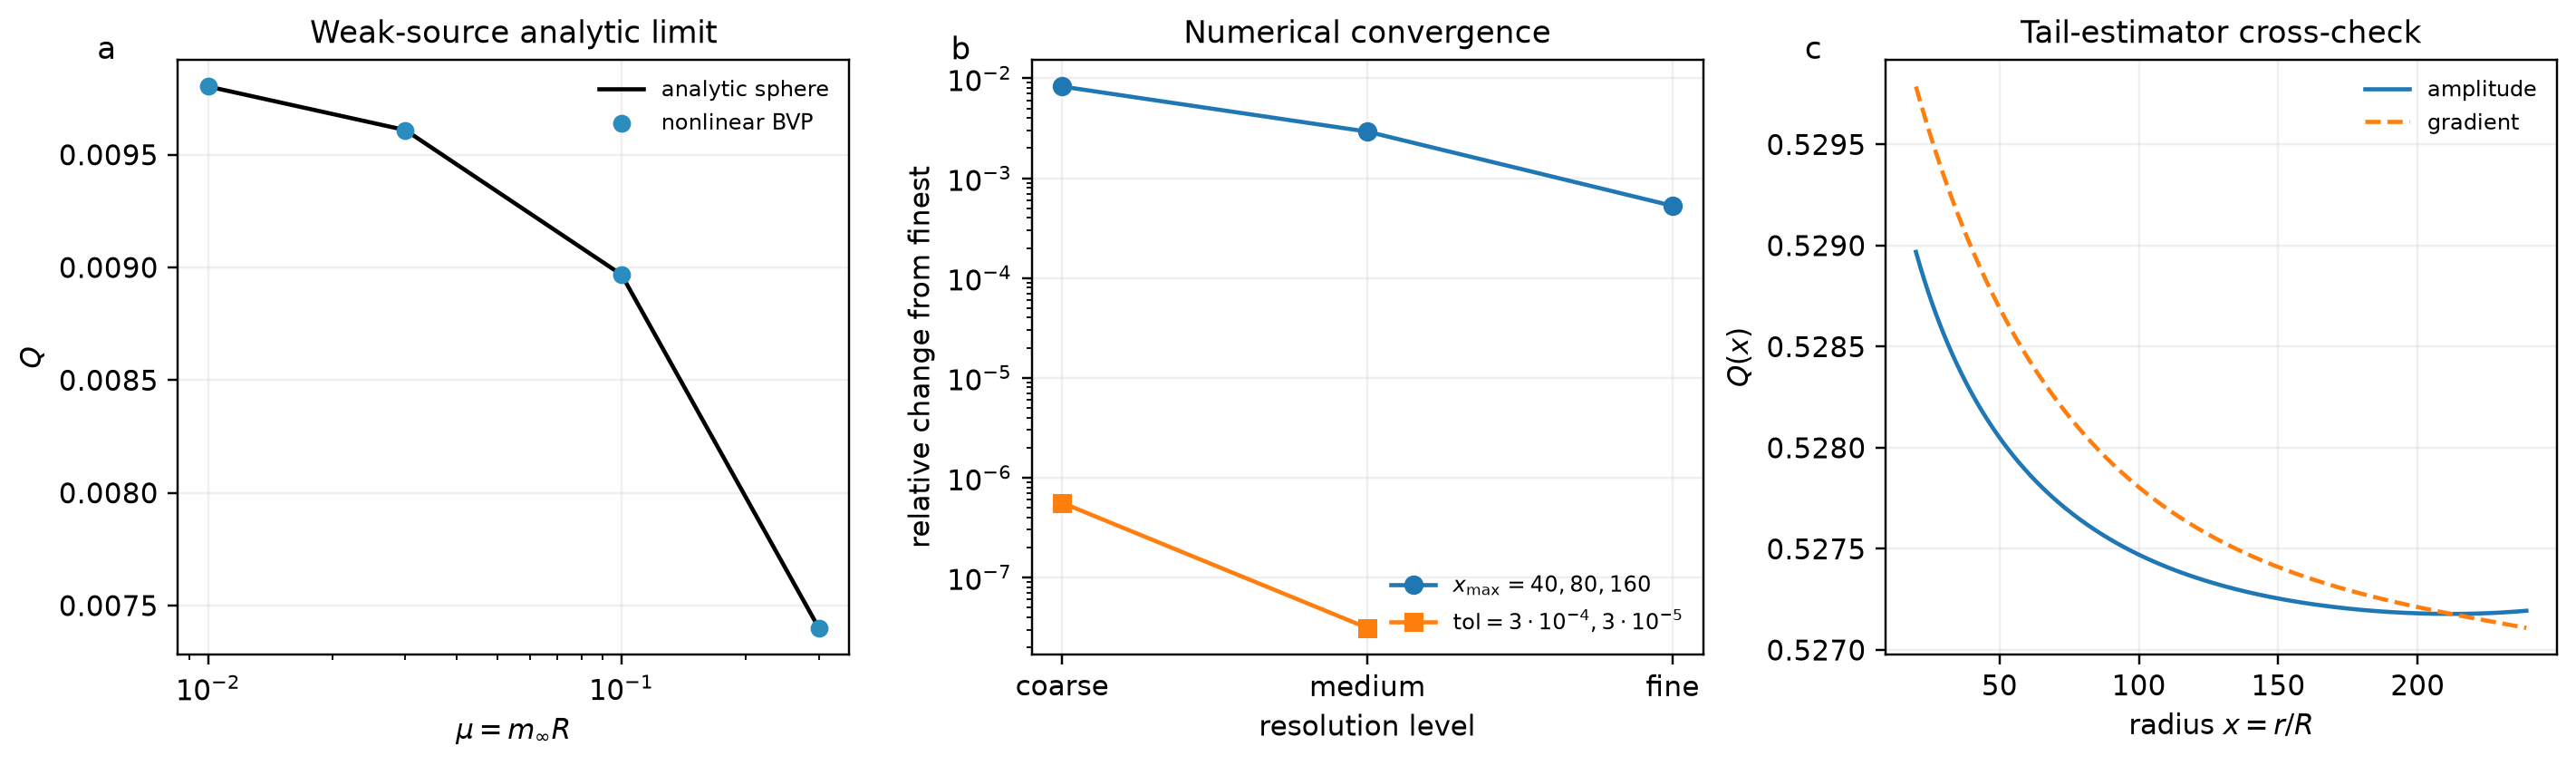
\includegraphics[width=.96\textwidth]{verification.png}
 \vspace{.05cm}
 \small
 Refined audit: \StudyAuditPoints\ points, including local-force threshold flips.\\[4pt]
 Charge change: at most \StudyAuditChargeMax\%. Local-force scan/refined difference:
 at most \StudyAuditForceMax\%.\\[3pt]
 Direct-force decision changes in the audit: \textbf{\StudyAuditForceFlips}.
\end{frame}

\begin{frame}{6. The field and its asymptotic charge}
 \centering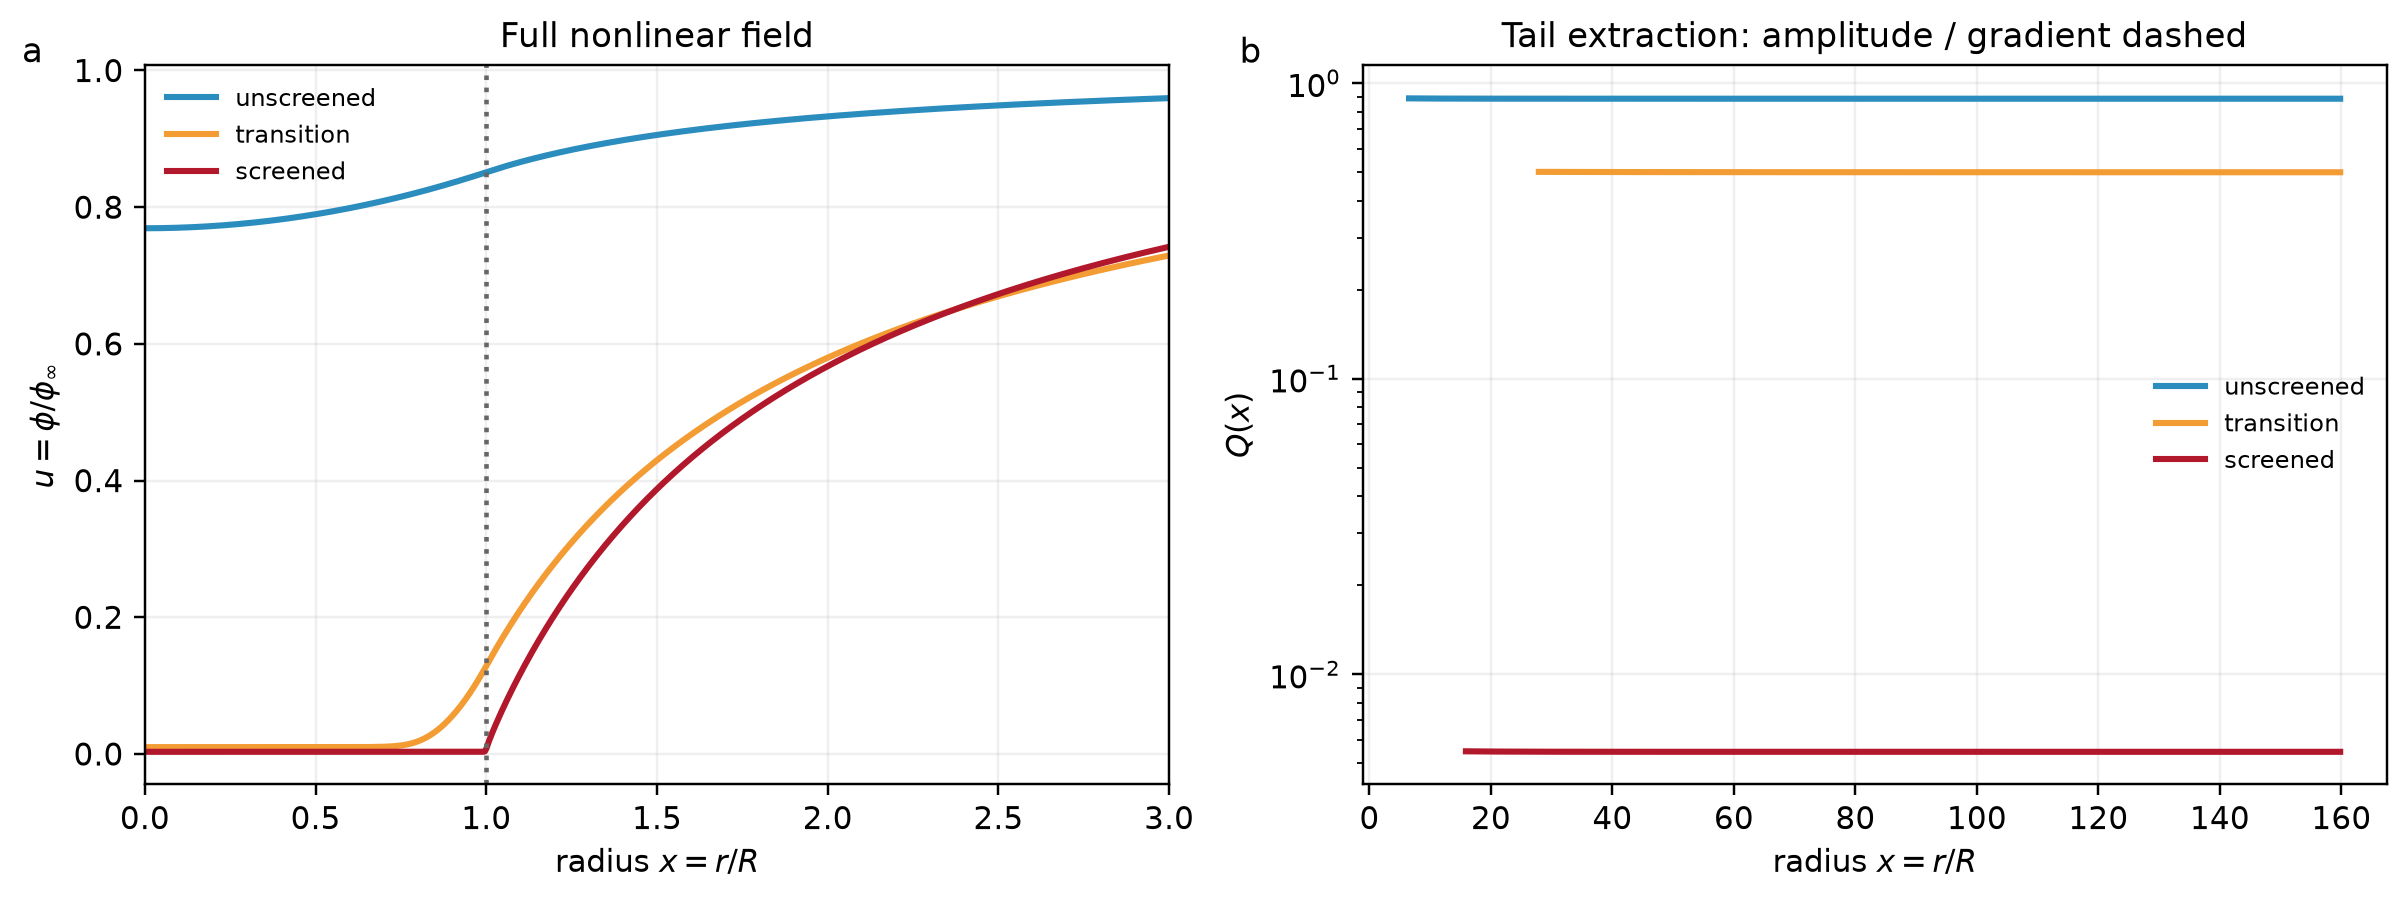
\includegraphics[width=.92\textwidth]{profiles_and_charge_extraction.png}
 \vspace{.05cm}
 \parbox{.94\textwidth}{\centering\small
 The far-tail amplitude and gradient estimators agree.\\[3pt]
 That agreement checks charge extraction, not near-source linearity.}
\end{frame}

\begin{frame}{7. Charge accuracy on the parameter grid}
 \centering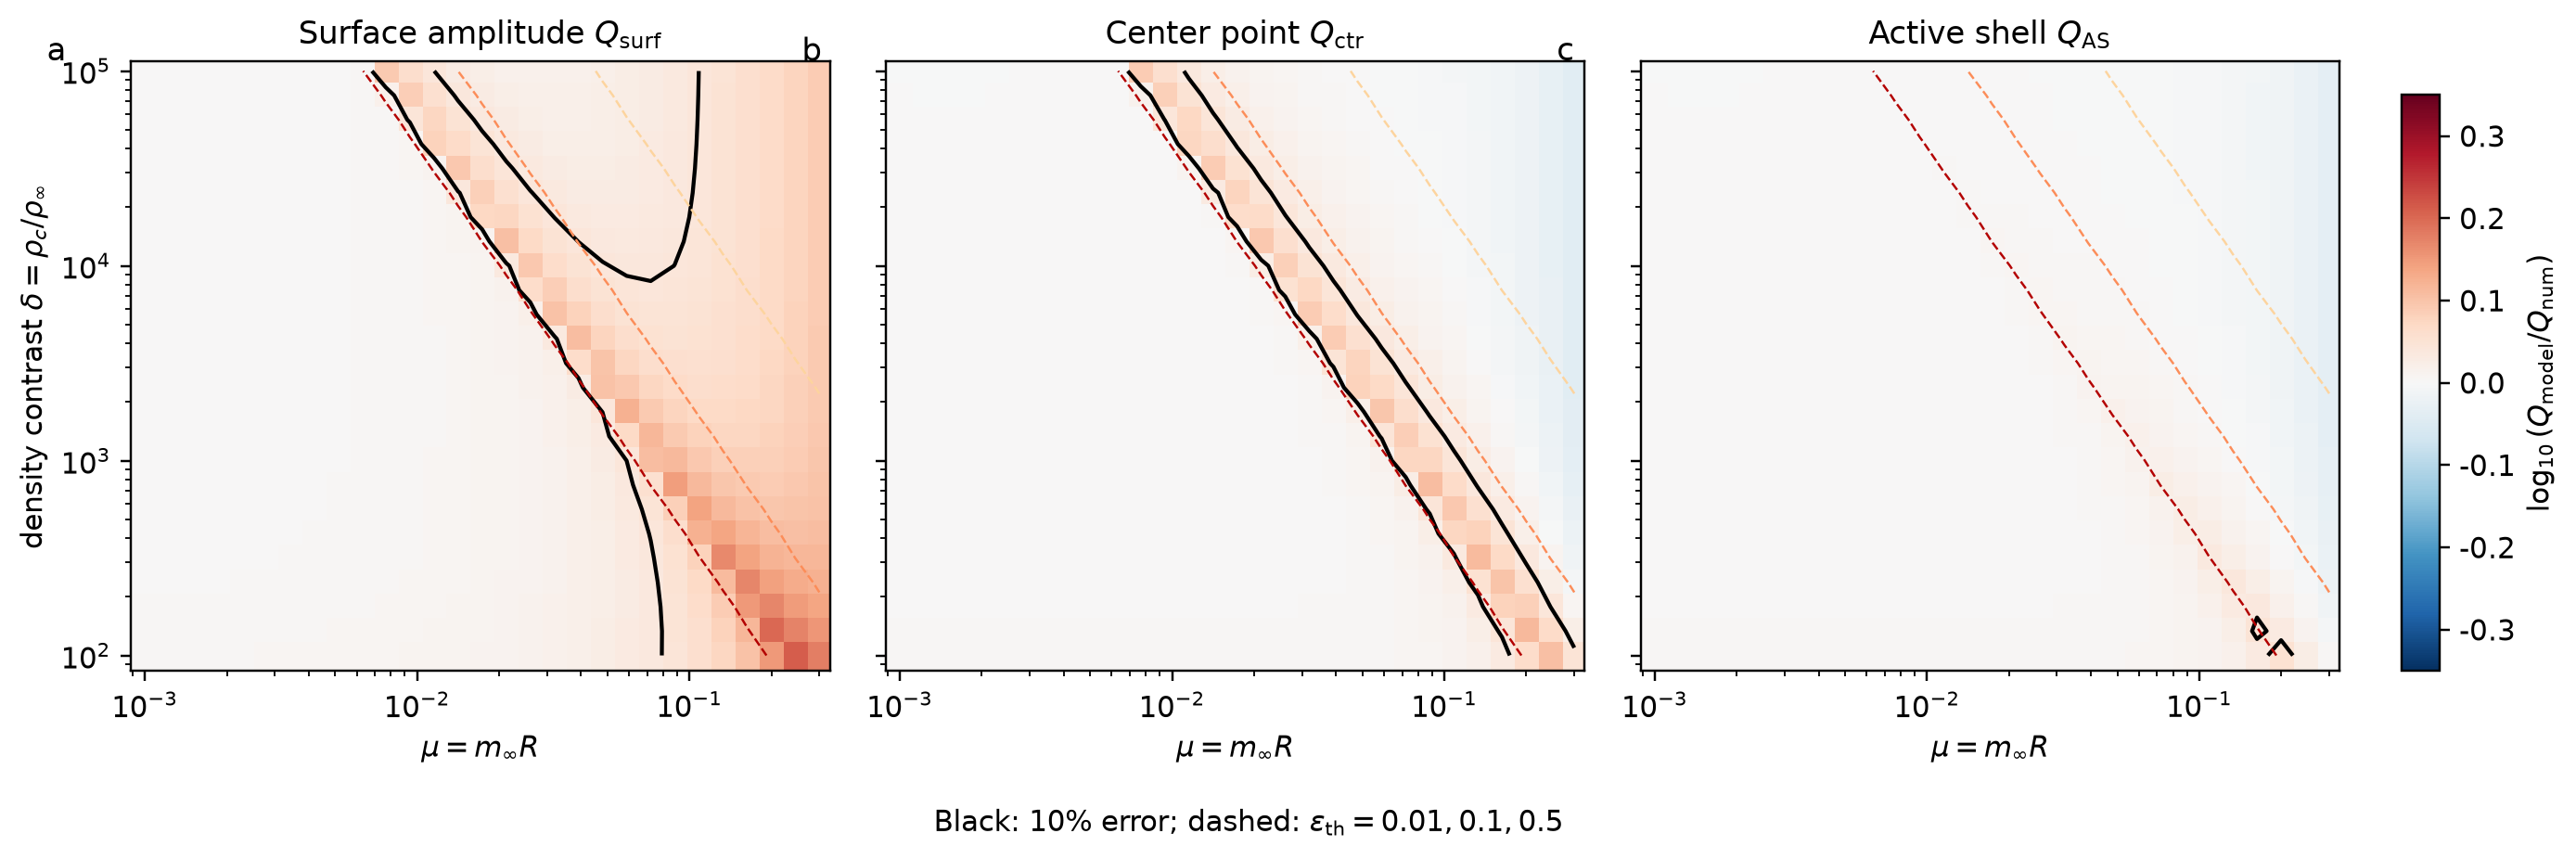
\includegraphics[width=.97\textwidth]{accuracy_atlas.png}
 \vspace{.06cm}
 \small
 10\% charge coverage: surface \StudySurfaceWithin\%, center \StudyCenterWithin\%,
 active shell \StudyASWithin\%.\\[3pt]
 These are fractions of the chosen grid, not probabilities for a theory.
\end{frame}

\begin{frame}{8. The simpler control reaches the same charge coverage}
 \centering\small
 \begin{tabular}{lrrr}\toprule
 Model & Median error & Maximum & Within 10\%\\\midrule
 \StudyChargeRowsEN
 \bottomrule\end{tabular}
 \vspace{.35cm}
 \[\qpv=e^{-\mu}\qms\qquad\hbox{versus}\qquad\qas\]
 \begin{itemize}
  \item Additional radial weighting changes the control by at most \StudyRadialMax\% here.
  \item Both reach \StudyASWithin\% coverage; radial weighting is not established as necessary.
 \end{itemize}
\end{frame}

\begin{frame}{9. Even the numerical charge can mispredict local force}
 \centering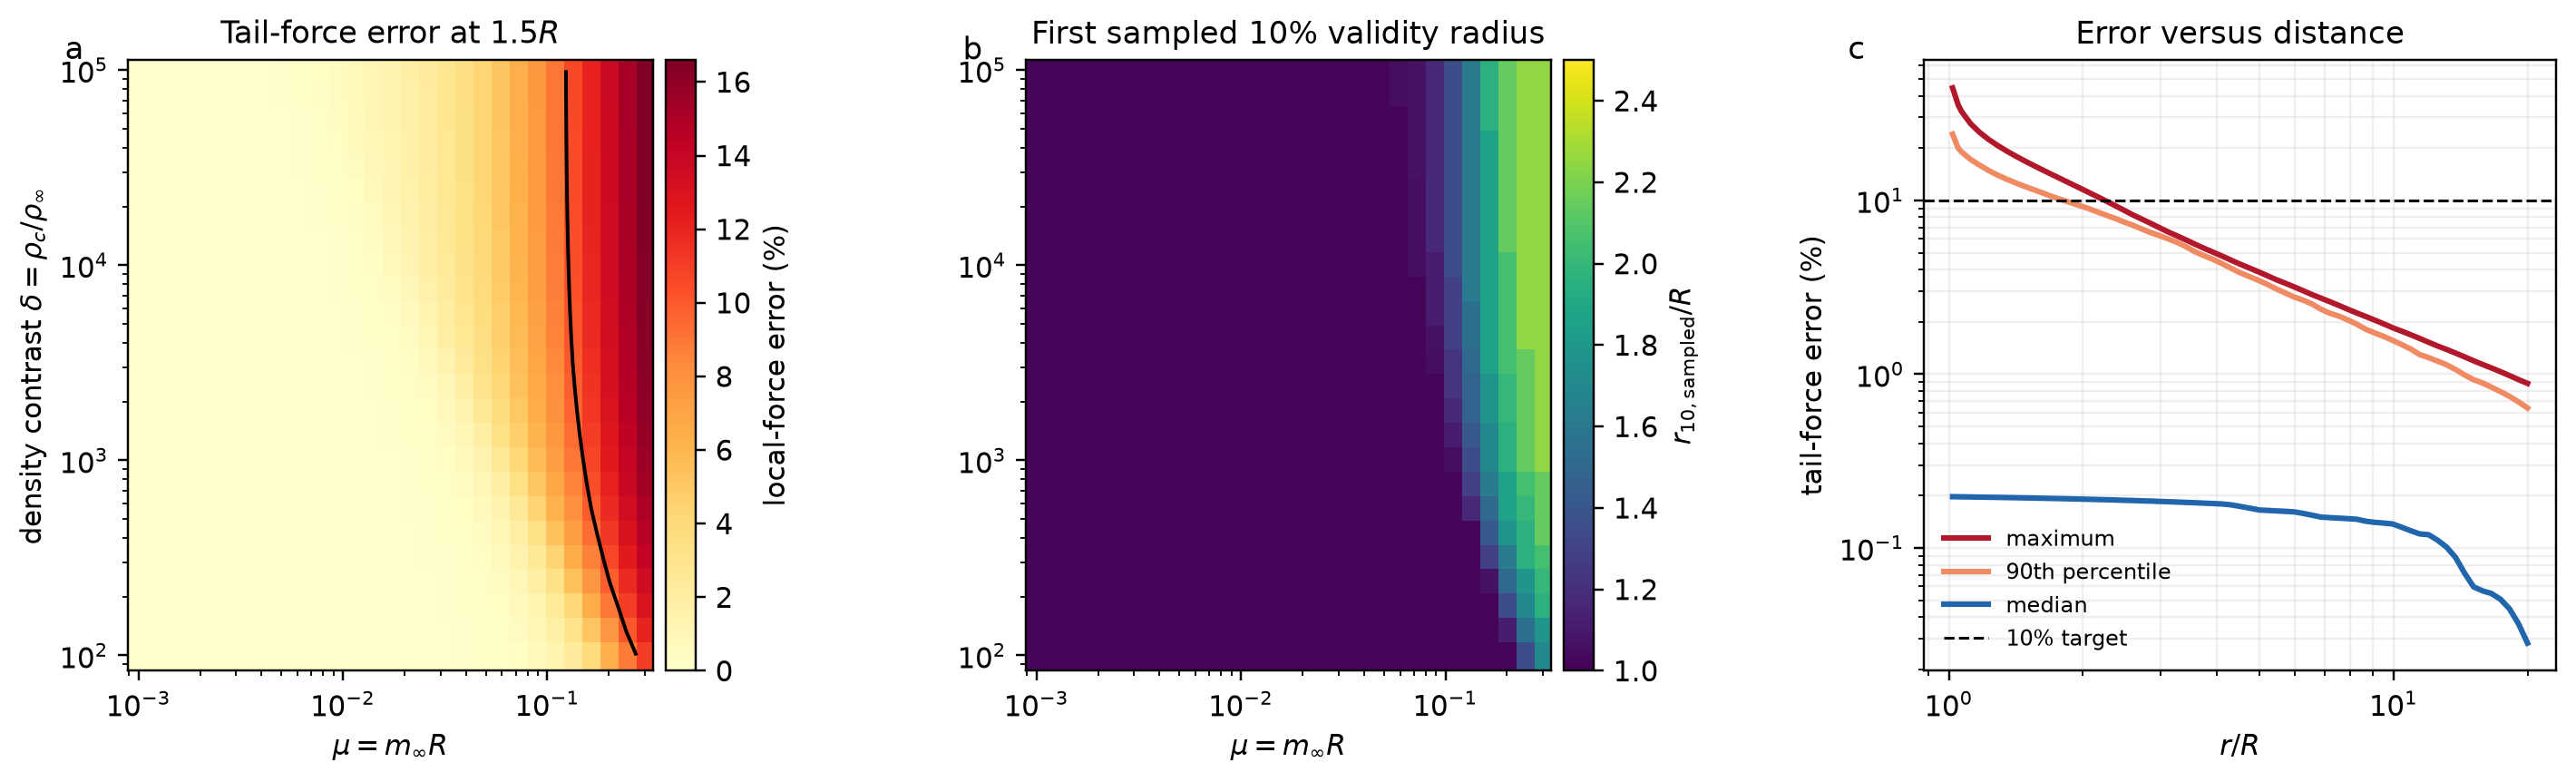
\includegraphics[width=.97\textwidth]{force_validity_map.png}
 \vspace{.05cm}
 \small
 Worst tail-force error: \textbf{\StudyForceNearMax\% at $1.5R$},
 \StudyForceFiveMax\% at $5R$, \StudyForceTenMax\% at $10R$.\\[3pt]
 The first-validity radius tests every later sampled radius through $20R$.
\end{frame}

\begin{frame}{10. Threshold map corrected to the direct force}
 \centering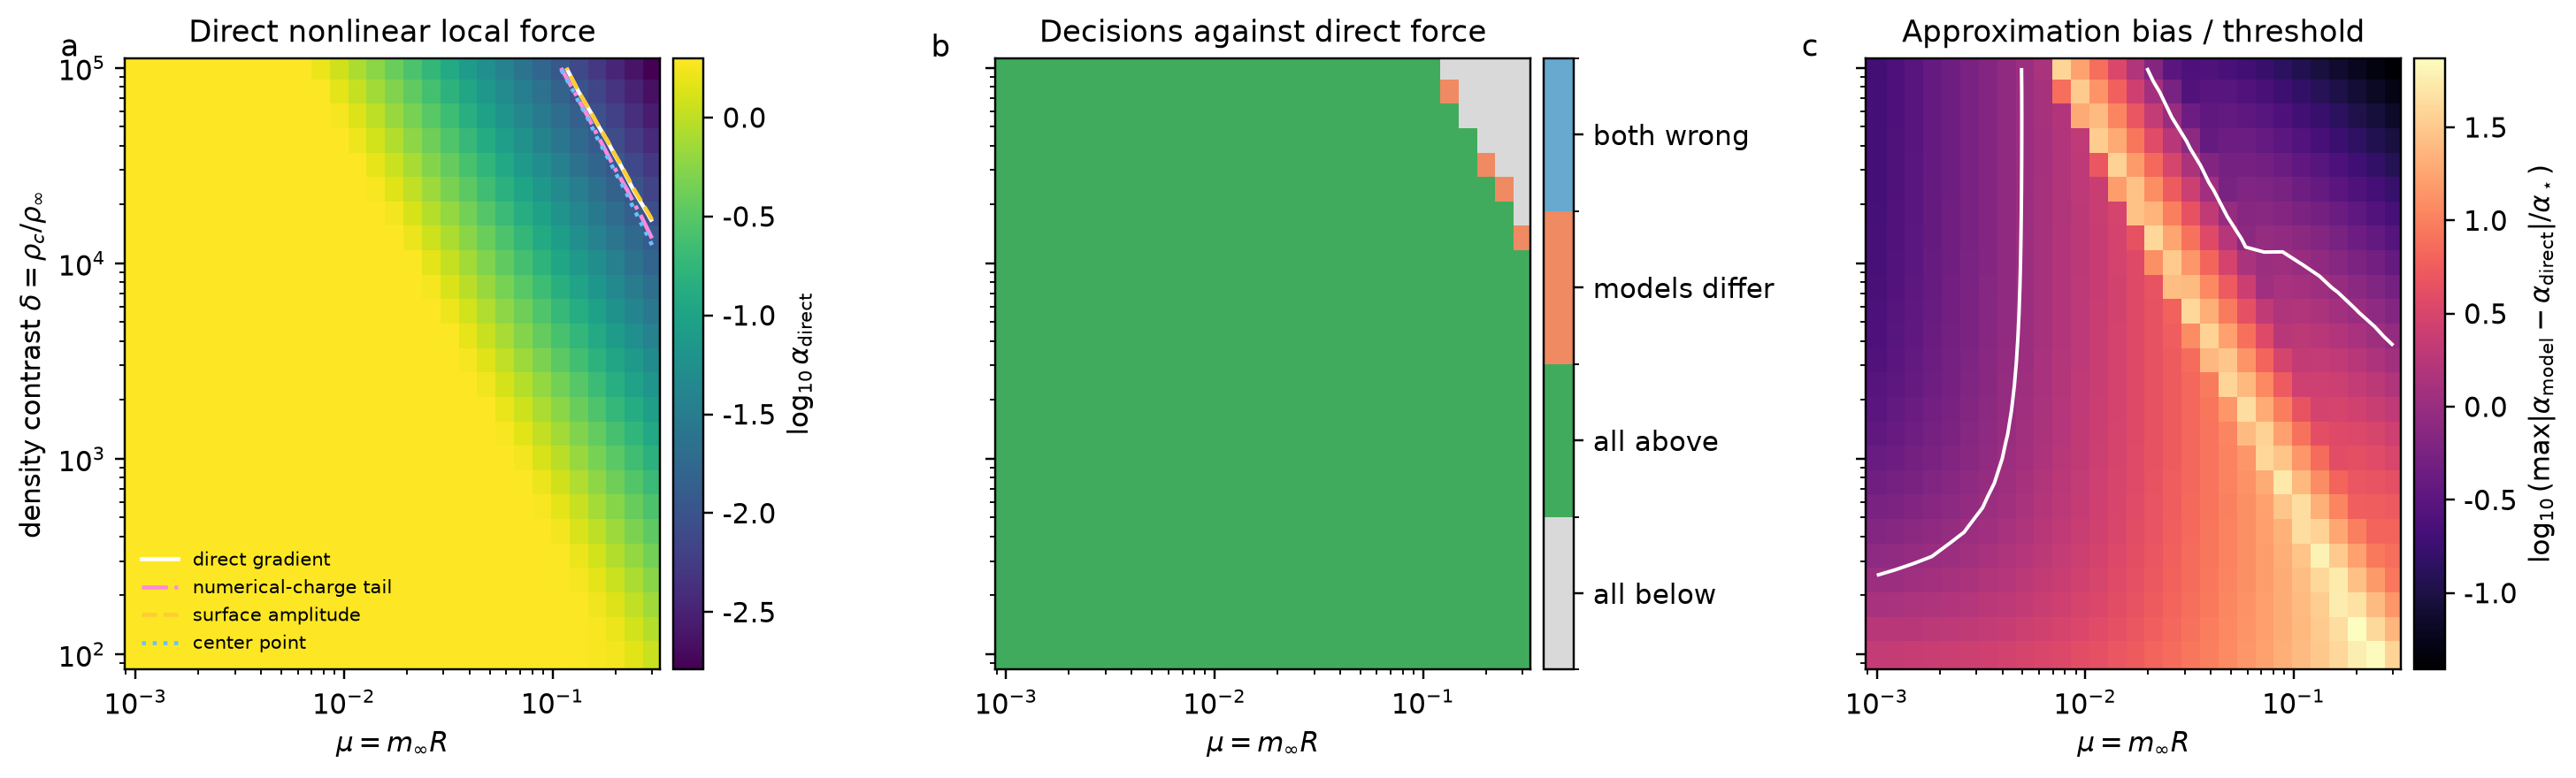
\includegraphics[width=.97\textwidth]{detectability_map.png}
 \vspace{.05cm}
 \small
 $\beta=Q_t=1$, $r=1.5R$, illustrative threshold $\alpha_\star=\StudyThreshold$.\\[3pt]
 Numerical-charge tail: \StudyTailFlips\ wrong decisions.
 Surface / center models: \StudySurfaceFlips\ / \StudyCenterFlips.\\[3pt]
 This is a local force-ratio map; apparatus scale and noise are not included.
\end{frame}

\begin{frame}{11. Error cancellation changes the observable ranking}
 \[\frac{\at(Q_j,x)}{\ad(x)}=
   \frac{Q_j}{\qnum}\frac{\at(\qnum,x)}{\ad(x)}\]
 \begin{columns}[T,onlytextwidth]
 \begin{column}{.47\textwidth}
  \begin{block}{Two errors multiply}
   A charge overestimate can partly cancel a near-field tail underestimate.
   Charge accuracy alone does not rank local-force predictions.
  \end{block}
  \small Active-shell 10\% coverage:\\
  charge \StudyASWithin\%, force at $1.5R$ \StudyASLocalWithin\%.
 \end{column}
 \begin{column}{.49\textwidth}
  \small
  \begin{itemize}
   \item Test several force-ratio thresholds; no crossing is a valid result.
   \item Distance validity is conditional on this $n=1$, $D\to0$ spherical grid.
   \item Real detectability also needs geometry, modulation, probe response, and noise.
  \end{itemize}
 \end{column}
 \end{columns}
\end{frame}

\begin{frame}{12. What this study establishes}
 \begin{enumerate}
  \item Specified charge models can be benchmarked reproducibly against a nonlinear BVP.
  \item The ablation limits the causal claim for radial weighting on this grid.
  \item A local gradient reference reveals a distance-dependent propagation error.
  \item The corrected force changes \StudyTailFlips\ decisions at $\alpha_\star=\StudyThreshold$.
 \end{enumerate}
 \vspace{.2cm}
 \begin{block}{Next research question}
  How does this charge-to-force validity change for $\mu\gtrsim1$,
  chamber walls, or different source shapes?
 \end{block}
 \centering\small
 \href{https://github.com/Lasqui-Ponto/Mechanics_Term_Project/tree/agent/improve-chameleon-project/Thin_Shell_Study}{Code, data, tests, and both language editions on GitHub}
\end{frame}

\begin{frame}{Selected references}
 \footnotesize
 \begin{thebibliography}{9}
 \bibitem{KW} J. Khoury and A. Weltman, \emph{Phys. Rev. Lett.} 93, 171104 (2004); \emph{Phys. Rev. D} 69, 044026 (2004).
 \bibitem{TT} T. Tamaki and S. Tsujikawa, \emph{Phys. Rev. D} 78, 084028 (2008).
 \bibitem{Review} C. Burrage and J. Sakstein, \emph{Living Rev. Relativ.} 21, 1 (2018).
 \bibitem{Elder} B. Elder et al., \emph{Phys. Rev. D} 94, 044051 (2016).
 \bibitem{Schlogel} S. Schl\"ogel et al., \emph{Phys. Rev. D} 93, 104036 (2016).
 \bibitem{Atom} D. Sabulsky et al., \emph{Phys. Rev. Lett.} 123, 061102 (2019).
 \bibitem{Yin} P. Yin et al., \emph{Nature Phys.} 18, 1181--1185 (2022).
 \end{thebibliography}
 \vfill\scriptsize Full derivations, limitations, and reproduction instructions are in the report.
\end{frame}
\end{document}
